
% Theophylline: pourquoi remontée de CL et de beta_CL sur les graphes après la barre rouge...
% Aussi: essai en changeant le nb d'itérations et sur un certain nb de runs, omega(ka)->0...

% Height of Oxford boys
% modèle linéaire vs modèle non-linéaire ???

% Yield model
% vérifier la vraisemblance des deux modèles et si on peut comparer les 2
% faire un test LRT entre 2 modèles ???

% ECO TODO à montrer
% graphes de convergence : interprétation
% utilisation de SAEM pour comparer des modèles
% utilisation des fonctions graphiques pour explorer les covariables
% différents scénarios (eg avec ou sans calcul des paramètres individuels, sans=les vaches ?)
% comparaison des différentes vraisemblances (lin, IS, GQ): fait

\chapter{Examples} \label{chapter_example} \label{sec:examples}

\section{Theophylline pharmacokinetics} \label{sec:exampletheo}

\subsection{One-compartment model}

Boeckmann, Sheiner and Beal (1994) report data from a study by Dr. Robert Upton of the kinetics of the anti-asthmatic drug theophylline~\cite{NONMEM}. Twelve subjects were given oral doses of the anti-asthmatic drug theophylline, then serum concentrations (in mg/L) were measured at 11 time points over the next 25 hours. In the present package, we removed the data at time 0 to avoid some unexplained non-zero values in a supposedly single-dose study. In the original dataset shipped with the {\sf NONMEM}, doses are given as doses per kilo body weight. Here, we therefore also transformed the doses to doses in mg instead of mg/kg.

These data are analyzed in Davidian and Giltinan~\cite{Davidian95} and Pinheiro and Bates~\cite{Pinheiro95} using a two-compartment open pharmacokinetic model. These data are also available in \R~in the library {\sf datasets} under the name {\sf Theoph} in a slightly modified format and including the data at time 0.

Subject $i$ receives an initial dose $D_i$ at time 0 and serum concentrations $y_{ij}$ are measured at time $t_{ij}$. Serum concentration is modeled by a first-order one compartment model, according to the following equation:
\begin{equation}
y_{ij} = \frac{\D D_i k_{ai} k_{ei}}{CL_i (k_{ai} - k_{ei})} \; \left( e^{-k_{ai} t_{ij}} - e^{-k_{ei} t_{ij}} \right) + \epsilon_{ij}
\end{equation}
where $CL_i$ is the clearance of subject $i$, $k_{ai}$ is the absorption rate constant, $k_{ei}$ is the elimination rate constant and is expressed as a function of $CL_i$ and the volume of distribution $V_i$ as $k_{ei}=\frac{CL_i}{V_i}$. For subject $i$:
\begin{itemize}
\item the vector of regression (or design) variables is $x_{ij} = (D_i , t_{ij} )$
\item the vector of individual parameters is $\theta_i = \left(\ln(k_{ai} ), \ln(CL_i), \ln(V_i) \right)$
   \begin{itemize}
   \item $k_{ai}$, $CL_{i}$ and $V_i$ are assumed to be independant log-normal random variables
   \item we assumed a relationship between the clearance and the subject's body weight ${\rm BW}_i$
   \end{itemize}
\begin{equation}
\begin{split}
\ln(k_{ai}) &= \mu_1 + \eta_1 \\
\ln(V_{i}) &= \mu_2 + \eta_2 \\
\ln(CL_{i}) &= \mu_3 + \beta {\rm BW}_i + \eta_3 \\
\end{split}
\end{equation}
\item we can use a simple homoscedastic error model where $\var{\epsilon_{ij}}=a^2$
\end{itemize}

The data is shown in figure~\ref{fig:theodata}.

\begin{figure}[!h]
\begin{center}
\par \kern -1cm
\epsfig{file=figs/theo_rawdata.eps,width=12cm,angle=270}
\end{center}
\par \kern -0.5cm
\caption{Theophylline concentrations versus time for the 12 subjects included in the study.} \label{fig:theodata}
\end{figure}

The following code was used in \R~to read the data and model:
\begin{verbatim}
library(saemix)

data(theo.saemix)
saemix.data<-saemixData(name.data=theo.saemix,header=TRUE,sep=" ",na=NA, 
name.group=c("Id"),name.predictors=c("Dose","Time"),name.response=c("Concentration"), 
name.covariates=c("Weight","Sex"),units=list(x="hr",y="mg/L",covariates=c("kg","-")), 
name.X="Time")

model1cpt<-function(psi,id,xidep) { 
	  dose<-xidep[,1]
	  tim<-xidep[,2]  
	  ka<-psi[id,1]
	  V<-psi[id,2]
	  CL<-psi[id,3]
	  k<-CL/V
	  ypred<-dose*ka/(V*(ka-k))*(exp(-k*tim)-exp(-ka*tim))
	  return(ypred)
}
saemix.model<-saemixModel(model=model1cpt,
description="One-compartment model with first-order absorption", 
psi0=matrix(c(1.,20,0.5,0.1,0,-0.01),ncol=3, byrow=TRUE,dimnames=list(NULL, 
c("ka","V","CL"))),transform.par=c(1,1,1), 
covariate.model=matrix(c(0,0,1,0,0,0),ncol=3,byrow=TRUE),fixed.estim=c(1,1,1),
covariance.model=matrix(c(1,0,0,0,1,0,0,0,1),ncol=3,byrow=TRUE), 
omega.init=matrix(c(1,0,0,0,1,0,0,0,1),ncol=3,byrow=TRUE), error.model="constant")
\end{verbatim}

In this example, we specify the vector of starting values through \texttt{psi0}, which is defined as the following matrix:
\begin{verbatim}
      ka  V    CL
[1,] 1.0 20  0.50
[2,] 0.1  0 -0.01
\end{verbatim}
The first line is renamed as Pop.CondInit when the model object is created (see output from the commands given in the snippet of code above), and contains the initial estimates of the population parameters $k_a$, $V$ and $CL$. The second line, renamed Cov.CondInit in this example, contains the initial values for the parameter-covariate relationships in the model. In this example, we have assumed an effect of the covariate Weight on the clearance $CL$, and the initial value of the corresponding fixed effect is -0.01. In this model there is no relationship between either of the two covariates in the model and $k_a$, so that the 0.1 value given in \texttt{psi0} will not be used. If we also had relationships between the covariate Sex and the model parameters, the same starting values would be used (using the vector recycling principle {\sf R}), however we could add other lines to \texttt{psi0} to specify different starting values. For example, assuming we want to estimate an effect of weight on $V$ and $CL$, as well as a gender effect on $CL$, we could replace the \texttt{covariate.model} argument with:
\begin{verbatim}
covariate.model=matrix(c(0,1,1,0,0,1),ncol=3,byrow=TRUE)
\end{verbatim}
and give different starting values for each parameter-relationship in \texttt{psi0}, for example 0.1 for both weight effects and -0.1 for the gender effect:
\begin{verbatim}
psi0=matrix(c(1.,20,0.5,0,0.1,0.1,0,0,-0.1),ncol=3, byrow=TRUE,dimnames=list(NULL, 
c("ka","V","CL")))
\end{verbatim}

Note that the model requires two predictors, dose and time. The user is responsible for writing the model function and checking the consistency between the model function and the data. Here, the first predictor (first column) is dose and the second predictor is time so that we need both items in the dataset, and we need to give the names of the two predictors in the proper order (the order corresponding to the way the model function is written here) when creating the data object. This is a single-dose administration and therefore the dose column contains the same dose repeated for each time-point. However, for graphs we want the observations to be plotted versus time and not versus dose; by default, the program will use the first predictor as the X axis, but we override this behaviour here by setting the option {\sf name.X="Time"} in the creation of the data object, so that the graphs will use time on the X-axis.

Then we fit the model using the {\sf saemix()} function:
\begin{verbatim}
saemix.fit<-saemix(saemix.model,saemix.data,list(seed=632545,nb.chains=5,
nbiter.saemix = c(300, 150)))
\end{verbatim}
We use 5 chains here to stabilise the estimation because there are only 12 subjects in the dataset (by default, the algorithm will increase the number of chains if there are less than 50 subjects in the dataset, and set it to a higher value as describe in section~\ref{sec:usingsaemix}), and we increase the number of steps in the second stage to 150 (default: 100) to show how to set this option. Increasing the number of iterations in the second stage helps to obtain a more stable conditional distribution for the individual parameters.

This produces the following output:
\begin{verbatim}
 ............
Nonlinear mixed-effects model fit by the SAEM algorithm
-----------------------------------
----          Data             ----
-----------------------------------
Object of class SaemixData
    longitudinal data for use with the SAEM algorithm
Dataset theo.saemix 
    Structured data: Concentration ~ Dose + Time | Id 
    X variable for graphs: Time (hr) 
    covariates: Weight (kg), Sex (-) 
First 10 lines of data:
   Id    Dose  Time Concentration Weight Sex
1   1 319.992  0.25          2.84   79.6   1
2   1 319.992  0.57          6.57   79.6   1
3   1 319.992  1.12         10.50   79.6   1
4   1 319.992  2.02          9.66   79.6   1
5   1 319.992  3.82          8.58   79.6   1
6   1 319.992  5.10          8.36   79.6   1
7   1 319.992  7.03          7.47   79.6   1
8   1 319.992  9.05          6.89   79.6   1
9   1 319.992 12.12          5.94   79.6   1
10  1 319.992 24.37          3.28   79.6   1
-----------------------------------
----          Model            ----
-----------------------------------
Nonlinear mixed-effects model
  Model function:  One-compartment model with first-order absorption
function(psi,id,xidep) { 
  dose<-xidep[,1]
  tim<-xidep[,2]  
  ka<-psi[id,1]
  V<-psi[id,2]
  CL<-psi[id,3]
  k<-CL/V
  ypred<-dose*ka/(V*(ka-k))*(exp(-k*tim)-exp(-ka*tim))
  return(ypred)
}
  Nb of parameters: 3 
      parameter names:  ka V CL 
      distribution:
     Parameter Distribution
[1,] ka        log-normal  
[2,] V         log-normal  
[3,] CL        log-normal  
  Variance-covariance matrix:
   ka V CL
ka  1 0  0
V   0 1  0
CL  0 0  1
  Error model: constant , initial values: a=1 
  Covariate model:
       ka V CL
Weight  0 0  1
    Initial values
       ka  V    CL
PopCI 1.0 20  0.50
CovCI 0.1  0 -0.01
-----------------------------------
----    Key algorithm options  ----
-----------------------------------
    Algorithms: MAP, FIM, LL by IS 
    Number of iterations:  K1=300, K2=150 
    Number of chains:  5 
    Seed:  632545 
    Number of MCMC iterations for IS:  5000 
    Simulations:
        nb of simulated datasets used for npde:  1000 
        nb of simulated datasets used for VPC:  100 
    Input/output
        save the results to file pop_parameters.txt in directory:  newdir 
        save graphs
-----------------------------------
----          Results          ----
-----------------------------------
----------------------------------------------------
-----------------  Fixed effects  ------------------
----------------------------------------------------
     Parameter       Estimate SE     CV(%) p-value
[1,] ka               1.567   0.2998  19.1 -      
[2,] V               31.475   1.3838   4.4 -      
[3,] CL               1.581   1.0155  64.2 -      
[4,] beta_Weight(CL)  0.008   0.0092 113.5 0.19   
[5,] a                0.743   0.0569   7.7 -      
----------------------------------------------------
-----------  Variance of random effects  -----------
----------------------------------------------------
   Parameter Estimate SE    CV(%)
ka omega.ka  0.388    0.175 45   
V  omega.V   0.015    0.009 59   
CL omega.CL  0.070    0.034 49   
----------------------------------------------------
------  Correlation matrix of random effects  ------
----------------------------------------------------
         omega.ka omega.V omega.CL
omega.ka 1        0       0       
omega.V  0        1       0       
omega.CL 0        0       1       
----------------------------------------------------
---------------  Statistical criteria  -------------
----------------------------------------------------
Likelihood computed by linearisation
      -2LL= 343.4919 
      AIC = 359.4919 
      BIC = 363.3712 

Likelihood computed by importance sampling
      -2LL= 344.8896 
      AIC = 360.8896 
      BIC = 364.7689 
----------------------------------------------------
\end{verbatim}
By default, the results are saved in a file called {\sf pop\_parameters.txt} in the {\sf newdir} directory, and graphs are produced.

Table~\ref{tab:paramtheo} reports the parameters obtained on a Linux Ubuntu distribution running \R~version 2.11.1 for this example. In this example, the fixed effect representing the influence of weight on CL is not significant (p=0.19, NS according to a Wald test).
\begin{table}[!h]
\begin{center}
\begin{tabular}{r c c}
\hline
Parameter & Population estimate & IIV Variance \\
& (SE\%) & (SE\%) \\
\hline
$k_{a}$ (hr$^{-1}$) & 1.57 (19\%) & 0.39 (45\%)\\
$CL$ (L.hr$^{-1}$) & 1.58 (64\%) & 0.07 (49\%) \\ 
$\beta_{BW,CL}$ (-) & 0.008 (110\%) & - \\
$V$ (L) & 31.5 (4\%) & 0.02 (59\%) \\
a (mg.L$^{-1}$) & 0.74 (6\%) & - \\
\hline
\end{tabular} 
\caption{Pharmacokinetic parameters estimated by \monolix~for the theophylline data.} \label{tab:paramtheo}
\end{center}
\end{table}

A series of diagnostic plots can be produced simply by applying the function {\sf plot() to the object returned by {\sf saemix()}:
\begin{verbatim}
plot(saemix.fit)
\end{verbatim}
By using the {\sf plot.type=""} argument, specific graphs can be produced (see section~\ref{sec:plot.functions}). For example, the convergence plot shown in figure~\ref{fig:convergtheo} can be produced by:
\begin{verbatim}
plot(saemix.fit,plot.type="convergence")
\end{verbatim}
In this figure we can see all the parameters converging quickly to their estimated value.

%ECO TODO: pourquoi ça remonte pour CL...

\begin{figure}[!h]
\begin{center}
\par \kern -1cm
\epsfig{file=figs/theo_convergence.eps,width=11cm,angle=270}
\end{center}
\par \kern -0.5cm
\caption{Convergence plots for the estimated pharmacokinetic parameters and the variabilities.} \label{fig:convergtheo}
\end{figure}

Figure~\ref{fig:LLIS} shows the evolution of the log-likelihood during the importance sampling step. Figure~\ref{fig:theodiagnos} shows the predicted values compared to the observed concentrations, for the population predictions (left) and the individual predictions (right). Figure~\ref{fig:theoindividual} shows the individual data for the 12 subjects, with the individual predictions overlayed (smoothed predictions were obtained). Both plots indicate good model adequacy.

\begin{figure}[!h]
\begin{center}
\par \kern -1cm
\epsfig{file=figs/theo_llis.eps,width=9cm,angle=270}
\end{center}
\par \kern -0.5cm
\caption{Estimating the log-likelihood by Importance Sampling.} \label{fig:LLIS}
\end{figure}

\begin{figure}[!h]
\begin{center}
\par \kern -0.2cm
\epsfig{file=figs/theo_diagnos.eps,width=10.5cm,angle=270}
\end{center}
\par \kern -0.8cm
\caption{Observations versus predictions (left: population predictions, right: individual predictions).} \label{fig:theodiagnos}
\end{figure}

\begin{figure}[!h]
\begin{center}
\par \kern -1cm
\epsfig{file=figs/theo_individualfits_smooth.eps,width=14.5cm,angle=0}
\end{center}
\par \kern -0.8cm
\caption{Individual plots for the 12 subjects in the study. Dots represent observations and the line shows the smoothed profile predicted using the individual estimated parameters.} \label{fig:theoindividual}
\end{figure}

\clearpage
\newpage

\bigskip
The following example shows how to use the functions defined in section~\ref{sec:plot.functions} to plot the individual fits for the first 4 subjects in the theophylline example, including a smoothed prediction line, and changing the color of the line and the plotting symbol. A logarithmic scale is used for the Y-axis. The resulting plot is shown in figure~\ref{fig:theoindopt}
\begin{figure}[!h]
\begin{center}
\epsfig{file=figs/theo_individualfits_smoothlog.eps,width=11.5cm,angle=270}
\end{center}
\par \kern -0.5cm
\caption{Individual plots for the first 4 subjects in the study, with different options.} \label{fig:theoindopt}
\end{figure}

To obtain these plots, we can use the generic function {\sf plot()}, by setting the {\sf plot.type} argument to "individual.fit", to produce these plots:
\begin{verbatim}
# Plotting individual fits with selected options
par(mfrow=c(2,2))
plot(saemix.fit,plot.type="individual.fit",new=FALSE,ilist=1:4,smooth=TRUE,ylog=T,
pch=1, col="Blue",xlab="Time in hr",ylab="Theophylline concentrations (mg/L)")
\end{verbatim}
We can also use directly the {\sf saemix.plot.fits()} function with the same graphical options, which gives the exact same graph:
\begin{verbatim}
# Plotting individual fits with selected options
par(mfrow=c(2,2))
saemix.plot.fits(saemix.fit,new=FALSE,ilist=1:4,smooth=TRUE,ylog=T,pch=1,
col="Blue",xlab="Time in hr",ylab="Theophylline concentrations (mg/L)")
\end{verbatim}

Other diagnostic plots include Visual Predictive Checks, shown in figure~\ref{fig:theovpc}, and residual plots. 
\begin{figure}[!h]
\par \kern -0.5cm
\begin{center}
\epsfig{file=figs/theo_VPC.eps,width=11.5cm,angle=270}
\end{center}
\par \kern -0.5cm
\caption{VPC for the theophylline data.} \label{fig:theovpc}
\end{figure}

The following code can be used to first simulate from the model in order to compute simulation-based metrics (residuals and VPC), and then produce VPC and scatterplots of residuals versus time and predictions (figure~\ref{fig:theoresid}).

\begin{verbatim}
# Scatterplots of residuals
plot(saemix.fit, plot.type="residuals.scatter")

# VPC
plot(saemix.fit, plot.type="vpc")
\end{verbatim}

\begin{figure}[!h]
\begin{center}
\par \kern -0.5cm
\epsfig{file=figs/theo_residscatter.eps,width=11.5cm,angle=270}
\end{center}
\par \kern -0.5cm
\caption{Scatterplots of the residuals (left: weighted population residuals; middle: individual weighted residuals; right: npde) versus time (top) and predictions (bottom).} \label{fig:theoresid}
\end{figure}

Finally, note that the SAEM algorithm is relatively robust to the initial choice of parameter estimates, but different initial choices may lead to different population estimates. Here, if we had set all the initial parameters to 1 as in the following code, the model converges to very different values and a flip-flop occurrs ($k_a$ becomes smaller than the elimination rate constant $k=CL/V$). The resulting fit however has a lower likelihood and the VPC graphs indicate poor estimates of the variability (not shown), which can give an indication of problems with the model.
\begin{verbatim}
saemix.model<-saemixModel(model=model1cpt,
description="One-compartment model with first-order absorption",
psi0=matrix(c(1.,1.,1.,0.1,0,-0.01),ncol=3, byrow=TRUE,dimnames=list(NULL, 
c("ka","V","CL"))),transform.par=c(1,1,1), 
covariate.model=matrix(c(0,0,1,0,0,0),ncol=3,byrow=TRUE), fixed.estim=c(1,1,1), 
covariance.model=matrix(c(1,0,0,0,1,0,0,0,1),ncol=3,byrow=TRUE), 
omega.init=matrix(c(1,0,0,0,1,0,0,0,1),ncol=3,byrow=TRUE), error.model="constant")
\end{verbatim}
Thus, it is always good policy during data analysis to check the stability of the final model estimates by changing the initial estimates and running the algorithm again, and to compare the magnitude of the parameter estimates with a reference, such as prior information or litterature values.

%\clearpage

\subsection{One-compartment model at steady-state}

In the theophylline example, we described the pharmacokinetics using the single-dose, first-order absorption and elimination model. The following code shows how to fit the same data with the same model at steady-state, assuming a 24~hours dosing interval:
\begin{verbatim}
data(theo.saemix)
# Include a column for the inter-dose interval (tau)
theo.saemix2<-cbind(theo.saemix,tau=24)
saemix.data2<-saemixData(name.data=theo.saemix2,header=TRUE,sep=" ",na=NA, 
  name.group=c("Id"),name.predictors=c("Dose","Time","tau"),
  name.response=c("Concentration"),name.covariates=c("Weight","Sex"),
  units=list(x="hr",y="mg/L",covariates=c("kg","-")), name.X="Time")
# Define the model for steady-state
modelSS<-function(psi,id,xidep) { 
   dose<-xidep[,1]
   tim<-xidep[,2]  
   tau<-xidep[,3]  
   ka<-psi[id,1]
   V<-psi[id,2]
   CL<-psi[id,3]
   k<-CL/V
   ypred<-dose*ka/(V*(ka-k))*(exp(-k*tim)/(1-exp(-k*tau))-
exp(-ka*tim)/(1-exp(-ka*tau)))
   return(ypred)
}
saemix.model2<-saemixModel(model=modelSS,
  description="One-compartment model with first-order absorption, Steady-state",
  psi0=matrix(c(1.,20,0.5,0.1,0,-0.01),ncol=3,byrow=TRUE, 
  dimnames=list(NULL, c("ka","V","CL"))),transform.par=c(1,1,1))
     
# Run SAEMIX again
saemix.options<-list(seed=632545)
saemix.fit2<-saemix(saemix.model2,saemix.data2,saemix.options)
\end{verbatim}

\section{Simulated pharmacodynamic model}\label{sec:examplePD}

A symposium dedicated to Comparison of Algorithms Using Simulated Data Sets and Blind Analysis, took place in Lyon, France, September 2004, organised by P. Girard and F. Mentr\'e. During this symposium, a blind comparison of several PK/PD modelling software was performed, using simulated datasets. This example uses two datasets simulated for this comparison.

The two datasets contain 100 individuals, each receiving 3 different doses:(0, 10, 90), (5, 25, 65) or (0, 20, 30). It is assumed that doses were given in a cross-over study with sufficient wash-out period to avoid a carry-over effect. Responses $y_{ij}$ have been simulated with an E$_{\rm max}$ model, a standard pharmacodynamic model:
\begin{equation}
y_{ij} = E_{0,i} \frac{\D D_{ij} E_{\rm max,i}}{D_{ij} + ED_{50,i}} + \epsilon_{ij}
\end{equation}

For subject $i$:
\begin{itemize}
\item the regression variable is the dose received $x_{ij} = (D_i)$
\item the vector of individual parameters is $\theta_i = \left(\ln(E_{0,i}), \ln(E_{{\rm max},i}), \ln(ED_{50,i}) \right)$
\item the only available covariate is the gender $w_i$ of the individual (0 for male and 1 for female)
\end{itemize}
The individual parameters were simulated assuming a log-normal distribution for all parameters, and a gender effect on $ED_{50,i}$:
\begin{equation}
\begin{split}
\ln(E_{0,i}) &= \ln(E_{0}) + \eta_{i1} \\
\ln(E_{{\rm max},i}) &= \ln(E_{\rm max}) + \eta_{i2} \\
\ln(ED_{50,i}) &= \ln(ED_{50}) + \beta w_i + \eta_{i3} \\
\end{split}
\end{equation}
In the simulations, the fixed effects were set to $\left(\ln(E_{O}), \ln(E_{{\rm max}}), \ln(ED_{50}) \right)=(24 , 100 , 12)$. The covariance matrix of the random effects was a diagonal matrix. The variances of the random effects were (0.12 , 0.26 , 0.05). The residual variance was a constant variance, with $a^2 = 20$. The two data sets were simulated with different values of $\beta$:
\begin{itemize}
\item the first dataset was simulated with a gender effect, $\beta=0.3$, and is available in the package under the name {\sf PD1.saem}
\item the second dataset was simulated under the null hypothesis, $\beta=0$, and is available in the package under the name {\sf PD2.saem}
\end{itemize}

The data is shown in figure~\ref{fig:PDdata}.

\begin{figure}[!h]
\begin{center}
\par \kern -1cm
\epsfig{file=figs/PD_rawdata.eps,width=12cm,angle=270}
\end{center}
\par \kern -0.5cm
\caption{Effect versus dose for the data simulated with an E$_{\rm max}$ model, with a gender effect on $ED_{50}$ (left) and without a gender effect (right).} \label{fig:PDdata}
\end{figure}

The following code was used in \R~to run this example on the first dataset:
\begin{verbatim}
library(saemix)
data(PD1.saemix)
data(PD2.saemix)
saemix.data1<-saemixData(name.data=PD1.saemix,header=TRUE,name.group=c("subject"), 
name.predictors=c("dose"),name.response=c("response"),name.covariates=c("gender"), 
units=list(x="mg",y="-",covariates="-"))

saemix.data2<-saemixData(name.data=PD2.saemix,header=TRUE,name.group=c("subject"), 
name.predictors=c("dose"),name.response=c("response"),name.covariates=c("gender"), 
units=list(x="mg",y="-",covariates="-"))

modelemax<-function(psi,id,xidep) {
# input:
#   psi : matrix of parameters (3 columns, E0, Emax, EC50)
#   id : vector of indices 
#   xidep : dependent variables (same nb of rows as length of id)
# returns:
#   a vector of predictions of length equal to length of id
  dose<-xidep[,1]
  e0<-psi[id,1]
  emax<-psi[id,2]
  e50<-psi[id,3]
  f<-e0+emax*dose/(e50+dose)
  return(f)
}
saemix.model<-saemixModel(model=modelemax,description="Emax model", 
psi0=matrix(c(20,300,20,0,0,0),ncol=3,byrow=TRUE,
dimnames=list(NULL,c("E0","Emax","EC50"))),transform.par=c(1,1,1), 
covariate.model=matrix(c(0,0,1),ncol=3,byrow=TRUE), 
fixed.estim=c(1,1,1),covariance.model=matrix(c(1,0,0,0,1,0,0,0,1),ncol=3,
byrow=TRUE),error.model="constant")

saemix.options<-list(directory=directory,algorithms=c(1,1,1),nb.chains=1, 
save=FALSE,save.graphs=FALSE)

# Fitting the model on the two PD datasets
saemix.fit1<-saemix(saemix.model,saemix.data1,saemix.options)
saemix.fit2<-saemix(saemix.model,saemix.data2,saemix.options)
\end{verbatim}

Table~\ref{tab:paramPD} shows the parameter estimates for the two datasets. The estimates for the three fixed effects are similar for both datasets, while the estimate of $\beta$ is close to the values simulated for both. For {\sf PD2.saemix}, the SE on $\beta$ is very large, as is the SE on the estimate of the variability of $EC_{50}$.
\begin{table}[!h]
\begin{center}
\begin{tabular}{r c c c c}
\hline
& \multicolumn{2}{c}{PD1.saemix} &\multicolumn{2}{c}{PD2.saemix} \\
Parameter & Estimate (SE\%) & IIV (SE\%)  & Estimate (SE\%) & IIV (SE\%)\\
\hline
$E_{0}$ (-) & 22.71 (5\%) & 0.13 (22\%) & 23.18 (5\%) & 0.16 (20\%)\\
$E_{\rm max}$ (-) & 106.46 (6\%) & 0.31 (15\%) & 96.14 (5\%) & 0.22 (15\%) \\ 
$EC_{50}$ (mg) & 11.25 (8\%) & 0.03 (55\%) & 12.38 (6\%) & 0.01 (151\%)\\
$\beta_{gender,EC_{50}}$ (-) & 0.35 (26\%) & - & -0.06 (116\%) & - \\
a (mg.L$^{-1}$) & 4.94 (8\%) & - & 4.67 (8\%) & - \\
\hline
\end{tabular} 
\caption{Pharmacokinetic parameters estimated by \monolix~for the simulated PD data.} \label{tab:paramPD}
\end{center}
\end{table}

The convergence plots are shown in figures~\ref{fig:convergPD1} and~\ref{fig:convergPD2}, where we can see $\beta$ converging to a non-zero value for the first dataset, while the estimate fluctuates around 0 for the second dataset. The Wald test performed for the fixed effect representing the effect of gender on $EC_{50}$ shows that this parameter is significantly different from 0 in the first dataset (p=6.10$^{-5}$).

\begin{figure}[!h]
\begin{center}
\par \kern -1cm
\epsfig{file=figs/PD1_convergence.eps,width=11cm,angle=270}
\end{center}
\par \kern -0.5cm
\caption{Convergence plots for the estimated pharmacokinetic parameters and the variabilities, for the first dataset.} \label{fig:convergPD1}
\end{figure}

\clearpage
\begin{figure}[!h]
\begin{center}
\par \kern -1cm
\epsfig{file=figs/PD2_convergence.eps,width=11cm,angle=270}
\end{center}
\par \kern -0.5cm
\caption{Convergence plots for the estimated pharmacokinetic parameters and the variabilities, for the second dataset.} \label{fig:convergPD2}
\end{figure}

\bigskip
Finally, figure~\ref{fig:PDindividual} shows the individual data for the first 12 subjects in the first dataset, with the individual predictions overlayed. A smoothed prediction was obtained. The model fits the data extremely well, which is unsurprising given that this is simulated data, with a rather small residual variability.

\begin{figure}[!h]
\begin{center}
\par \kern -1cm
\epsfig{file=figs/PD1_individualfits.eps,width=14cm,angle=0}
\end{center}
\par \kern -0.5cm
\caption{Individual plots for the 12 subjects in the first dataset ({\sf PD1.saemix}). Dots represent observations and the line shows the profile predicted using the individual estimated parameters.} \label{fig:PDindividual}
\end{figure}

\clearpage
\newpage


\section{Weight gain of cows} \label{sec:examplecow}

The data used in this example is the evolution of the weight (in kg) of 560 cows. The weight of each cow was recorded on 9 or 10 occasions. An exponential model was assumed to describe the weight gain with time:
\begin{equation}
y_{ij} = A_{i} \; \left( 1- B_i e^{-K_i t_{ij}} \right) + \epsilon_{ij}
\end{equation}

For subject $i$:
\begin{itemize}
\item the regression variable is the time (in days) $x_{ij} = (t_{ij})$
\item the vector of individual parameters is $\theta_i = \left(A_i, B_i, K_i) \right)$
\item there were 3 covariates in the file:
   \begin{enumerate}
   \item the year of birth (beetween 1988 and 1998)
   \item existence of a twin (no=1, yes=2)
   \item the rank of birth (beetween 3 and 7)
   \end{enumerate}
\end{itemize}

The data is shown in figure~\ref{fig:cowdata}.

\begin{figure}[!h]
\begin{center}
%\par \kern -1cm
\epsfig{file=figs/weightcow_rawdata.eps,width=11cm,angle=270}
\end{center}
%\par \kern -1cm
\caption{Weight gain of 560 cows recorded repeatedly over time.} \label{fig:cowdata}
\end{figure}

The following code was used in \R~to run this example:
\begin{verbatim}
library(saemix)
data(cow.saemix)
saemix.data<-saemixData(name.data=cow.saemix,header=TRUE,name.group=c("cow"), 
name.predictors=c("time"),name.response=c("weight"), 
name.covariates=c("birthyear","twin","birthrank"), 
units=list(x="days",y="kg",covariates=c("yr","-","-")))

growthcow<-function(psi,id,xidep) {
# input:
#   psi : matrix of parameters (3 columns, ka, V, CL)
#   id : vector of indices 
#   xidep : dependent variables (same nb of rows as length of id)
# returns:
#   a vector of predictions of length equal to length of id
  x<-xidep[,1]
  a<-psi[id,1]
  b<-psi[id,2]
  k<-psi[id,3]
  f<-a*(1-b*exp(-k*x))
  return(f)
}
saemix.model<-saemixModel(model=growthcow,description="Exponential model",  
psi0=matrix(c(700,0.9,0.02,0,0,0),ncol=3,byrow=TRUE, 
dimnames=list(NULL,c("A","B","k"))),transform.par=c(1,1,1),fixed.estim=c(1,1,1), 
covariate.model=matrix(c(0,0,0,0,0,0,0,0,0),ncol=3,byrow=TRUE), 
covariance.model=matrix(c(1,0,0,0,1,0,0,0,1),ncol=3,byrow=TRUE), 
omega.init=matrix(c(1,0,0,0,1,0,0,0,1),ncol=3,byrow=TRUE),error.model="constant")

saemix.options<-list(algorithms=c(1,1,1),nbiter.saemix=c(200,100),nb.chains=1,
save=FALSE,save.graphs=FALSE)

# Fitting the models
saemix.fit<-saemix(saemix.model,saemix.data,saemix.options)
\end{verbatim}

\par \kern -0.2cm
As an alternative, we can compute the estimate of the likelihood by Gaussian Quadrature:
\begin{verbatim}
saemix.fit<-llgq.saemix(saemix.fit)
\end{verbatim}
%saemix.fit["results"]["ll.gq"]*(-2)
The three estimates of the likelihood were found to be in good agreement in this example:
\begin{verbatim}
----------------------------------------------------
---------------  Statistical criteria  -------------
----------------------------------------------------
Likelihood computed by linearisation
      -2LL= 53723.42 
      AIC = 53737.42 
      BIC = 53767.71 

Likelihood computed by importance sampling
      -2LL= 53723.88 
      AIC = 53737.88 
      BIC = 53768.18 

Likelihood computed by Gaussian quadrature
      -2LL= 53723.04 
      AIC = 53737.04 
      BIC = 53767.34 
----------------------------------------------------
\end{verbatim}

\bigskip
The fits to the data from the first 4 animals can be plotted using the function {\sf saemix.plot.fits}. First, default plot options are set in a list called {\sf saemix.plot.options} using the function  {\sf saemix.plot.setoptions}. Second, the option controlling the list of subjects to be plotted is set (here, we choose to plot the graphs for the first four animals), and the option {\sf smooth} indicates that we want an smoothed version of the plots (using interpolated weights):
\begin{verbatim}
plot(saemix.fit,plot.type="individual.fit",ilist=1:4,smooth=TRUE)
\end{verbatim}
The result is shown in figure~\ref{fig:cow.individual}.
\newpage
\begin{figure}[!h]
\begin{center}
\epsfig{file=figs/cow_indivfit4.eps,width=11cm,angle=270}
\end{center}
\par \kern -0.5cm
\caption{Fit for the first four subjects in the {\sf cow} dataset.} \label{fig:cow.individual}
\end{figure}

\section{Height of Oxford boys} \label{sec:exampleoxboys}

\monolix~can be used even for linear models. The dataset {\sf oxboys.saemix} was taken from the library {\sf nlme}~\cite{nlme}. It describes the evolution with age of the height of boys from Oxford, England. There is no covariate in the model, and we use a simple linear model to account for the increase in height over this age range:
\begin{equation}
y_{ij} = {\rm Base}_i + {\rm Slope} \; {\rm age}_{ij} + \epsilon_{ij}
\end{equation}
where ${\rm Base}_i$ is the baseline height at the entrance of subject $i$ in the study and ${\rm Slope}_i$ the slope for the increase of height with age ${\rm age}_{ij}$. For subject $i$:
\begin{itemize}
\item the vector of regression (or design) variables is $x_{ij} = ({\rm age}_{ij} )$
\item the vector of individual parameters is $\theta_i = \left( {\rm Base}_i, {\rm Slope}_i \right)$
   \begin{itemize}
   \item the individual parameters are assumed to have a normal distribution
   \end{itemize}
\item we can use a simple homoscedastic error model where $\var{\epsilon_{ij}}=a^2$
\end{itemize}

The data is shown in figure~\ref{fig:oxboysdata}.

\begin{figure}[!h]
\begin{center}
\par \kern -1cm
\epsfig{file=figs/oxboys_rawdata.eps,width=11cm,angle=270}
\end{center}
\par \kern -0.5cm
\caption{Evolution with age of the height of boys from Oxford.} \label{fig:oxboysdata}
\end{figure}

The following code was used in \R~to run this example:
\begin{verbatim}
library(saemix)

data(oxboys.saemix)
saemix.data<-saemixData(name.data=oxboys.saemix,header=T,name.group=c("Subject"), 
name.predictors=c("age"),name.response=c("height"), units=list(x="-",y="yr"))

growth.linear<-function(psi,id,xidep) {
# input:
#   psi : matrix of parameters (2 columns, base and slope)
#   id : vector of indices 
#   xidep : dependent variables (same nb of rows as length of id)
# returns:
#   a vector of predictions of length equal to length of id
  x<-xidep[,1]
  base<-psi[id,1]
  slope<-psi[id,2]
  f<-base+slope*x
  return(f)
}
saemix.model<-saemixModel(model=growth.linear,description="Linear model", 
psi0=matrix(c(140,1),ncol=2,byrow=T,dimnames=list(NULL,c("base","slope"))),  
transform.par=c(1,0), covariance.model=matrix(c(1,1,1,1),ncol=2,byrow=T), 
error.model="constant")

saemix.options<-list(algorithms=c(1,1,1),nb.chains=1)

saemix.fit<-saemix(saemix.model,saemix.data,saemix.options)
\end{verbatim}

%\clearpage
%\newpage

\par \kern -0.5cm
\section{A yield model} \label{sec:exampleyield}

The data used in this study were from 37 winter wheat experiments carried out between 1990 and 1996 on commercial farms in the Paris Basin, France. Each experiment was from a different site. Two soil types were represented, a loam soil and a chalky soil. Common winter wheat varieties were used. Each experiment consisted of five to eight different nitrogen fertilizer rates, for a total of 224 nitrogen treatments. Nitrogen fertilizer was applied in two applications during the growing season. For each nitrogen treatment, grain yield (adjusted to 150 g.kg$^{-1}$ grain moisture content) was measured. In addition, end-of-winter mineral soil nitrogen (NO3- plus NH4+) in the 0- to 90-cm layer was measured on each site-year during February when the crops were tillering. See [9] for a more complete description of the plant sampling and nitrogen analysis. Yield and end-of-winter mineral soil nitrogen measurements were in the ranges 3.44- 11.54 t.ha$^{-1}$ , and 40-180 kg.ha$^{-1}$ respectively.

The data is shown in figure~\ref{fig:yielddata}.
\begin{figure}[!h]
\begin{center}
\par \kern -1cm
\epsfig{file=figs/yield_rawdata.eps,width=11.5cm,angle=270}
\end{center}
\par \kern -0.5cm
\caption{Yield from 37 winter wheat experiments.} \label{fig:yielddata}
\end{figure}

Let $y_{ij}$ denote the $j^{\rm th}$ measurement of the yield response in the $i^{\rm th}$ site-year when the nitrogen fertilizer dose $d_{ij}$ is applied. The only available covariate is the amount of soil mineral nitrogen at the end of winter ($w_ i$).

A first model is a linear-plus-plateau function (LP) defined by:
\begin{equation}
y_{ij} = \left\{ \begin{array}{l r}
Y_{max,i} + B_i (d_{ij} - X_{max,i}) & \text{if } d_{ij} \leq X_{max,i} \\
Y_{max,i}  & \text{if } d_{ij} \geq X_{max,i} \\
         \end{array}
\right.
\end{equation}
This model includes three individual random parameters, $\phi_i = \left( Y_{max,i}, X_{max,i}, B_i \right)$. $Y_{max,i}$ is the maximal yield value in the $i^{\rm th}$ site-year and $X_{max,i}$ is the fertilizer dose that maximizes yield. The three parameters were assumed to follow a normal distribution.

A second model is a square-root-plus-plateau function (QP) defined by:
\begin{equation}
y_{ij} = \left\{ \begin{array}{l r}
Y_{max,i} + B_i (\sqrt{d_{ij}} - \sqrt{X_{max,i}}) & \text{if } d_{ij} \leq X_{max,i} \\
Y_{max,i}  & \text{if } d_{ij} \geq X_{max,i} \\
         \end{array}
\right.
\end{equation}

We use the following code to run these two models:
\begin{verbatim}
library(saemix)

data(yield.saemix)
saemix.data<-saemixData(name.data=yield.saemix,header=TRUE,name.group=c("site"), 
name.predictors=c("dose"),name.response=c("yield"), name.covariates=c("soil.nitrogen"), 
units=list(x="kg/ha",y="t/ha", covariates=c("kg/ha")))

yield.LP<-function(psi,id,xidep) {
  x<-xidep[,1]
  ymax<-psi[id,1]
  xmax<-psi[id,2]
  slope<-psi[id,3]
  f<-ymax+slope*(x-xmax)
#  cat(length(f),"  ",length(ymax),"\n")
  f[x>xmax]<-ymax[x>xmax]
  return(f)
}

yield.QP<-function(psi,id,xidep) {
  x<-xidep[,1]
  ymax<-psi[id,1]
  xmax<-psi[id,2]
  slope<-psi[id,3]
  f<-ymax+slope*(x**0.5-xmax**0.5)
#  f<-ymax+slope*sqrt(abs(x-xmax))
  f[x>xmax]<-ymax[x>xmax]
  return(f)
}
saemix.model1<-saemixModel(model=yield.LP,description="Linear + plateau model",  
psi0=matrix(c(8,100,0.2,0,0,0),ncol=3,byrow=T, dimnames=list(NULL,c("Ymax","Xmax", 
"slope"))), covariate.model=matrix(c(0,0,0),ncol=3,byrow=T), 
transform.par=c(0,0,0),covariance.model=matrix(c(1,0,0,0,1,0,0,0,1),ncol=3,byrow=T), 
error.model="constant")

saemix.model2<-saemixModel(model=yield.QP,description="Quadratic + plateau model", 
psi0=matrix(c(10,120,0.005,0,0,0),ncol=3,byrow=T, dimnames=list(NULL,c("Ymax","Xmax", 
"slope"))), covariate.model=matrix(c(0,0,0),ncol=3,byrow=T), transform.par=c(0,0,0), 
covariance.model=matrix(c(1,0,0,0,1,0,0,0,1),ncol=3,byrow=T),error.model="constant")

saemix.options<-list(algorithms=c(1,1,1),nb.chains=1, nbiter.saemix=c(400,100), 
nmc.is=25000, save=FALSE,save.graphs=FALSE)

# Fitting the models
saemix.fit1<-saemix(saemix.model1,saemix.data,saemix.options)
saemix.fit2<-saemix(saemix.model2,saemix.data,saemix.options)
\end{verbatim}
The two models perform very similarly in terms of log-likelihood, with a slight advantage to the LP model: the statistical criterion (-2 times the log-likelihood) was equal to 406.86 for the LP model and to 416.28 for the QP model. Figure~\ref{fig:yielddiagnos} shows the plots of predictions versus observations for the two models, again very similar.

\newpage
\begin{figure}[!h]
\begin{center}
\par \kern -0.5cm
\epsfig{file=figs/yield_comparemodels_diagnos.eps,width=10cm,angle=270}
\end{center}
\par \kern -0.5cm
\caption{Observations versus predictions for the LP model (upper panel) and QP model (lower panel), with population predictions on the left and individual predictions on the right.} \label{fig:yielddiagnos}
\end{figure}

Figure~\ref{fig:yieldindiv} shows the fit of the two models for the first four subjects. The figure was obtained using the following code:
\begin{verbatim}
par(mfrow=c(4,2))
for(i in 1:4) {
  plot(saemix.fit1,plot.type="individual.fit",ilist=i,smooth=TRUE,new=F)
  plot(saemix.fit2,plot.type="individual.fit",ilist=i,smooth=TRUE,new=F)
}
\end{verbatim}

\begin{figure}[!h]
\begin{center}
\par \kern -1cm
\epsfig{file=figs/yield_comparemodels_indiv.eps,width=14cm,angle=0}
\end{center}
\par \kern -0.5cm
\caption{Fits for the LP model (left) and QP model (right) for the first 4 subjects.} \label{fig:yieldindiv}
\end{figure}
\clearpage

We can explore the covariates using diagnostic plots. For instance, the following code plots the estimated individual parameters versus the covariates in the model (here, soil nitrogen), assuming the fit is in the object saemix.fit:
\begin{verbatim}
plot(saemix.fit1, plot.type="parameters.vs.covariates")
\end{verbatim}
Figure~\ref{fig:yieldparcov} shows the result, and indicates a decreasing trend in $X_{max}$ with increasing amounts of soil nitrogen.
\begin{figure}[!h]
\begin{center}
\par \kern -1cm
\epsfig{file=figs/yield_parvscov.eps,width=11cm,angle=270}
\end{center}
\par \kern -0.5cm
\caption{Graphs of the estimated (individual) parameters versus covariate.} \label{fig:yieldparcov}
\end{figure}

In this example, we can then show with \monolix~that the effect of the amount of soil mineral nitrogen at the end of winter is statistically significant for explaining the fluctuations of the parameter $X_{max}$ in both LP and QP models, with a drop of over 20 points in the statistical criterion. For example, the following code shows how to fit the LP-model with and without covariate effect on X$_{\rm max}$, and outputs the resulting log-likelihoods:

\begin{verbatim}
saemix.model3<-saemixModel(model=yield.LP,description="Linear + plateau model",  
psi0=matrix(c(8,100,0.2,0,0,0),ncol=3,byrow=T, dimnames=list(NULL,c("Ymax","Xmax", 
"slope"))), covariate.model=matrix(c(0,1,0),ncol=3,byrow=T), 
transform.par=c(0,0,0),covariance.model=matrix(c(1,0,0,0,1,0,0,0,1),ncol=3,byrow=T), 
error.model="constant")

saemix.fit3<-saemix(saemix.model3,saemix.data,saemix.options)

{
  cat("LP model:\n")
  cat("     without covariate, -2xLL=",(saemix.fit1["results"]["ll.is"])*(-2),"\n")
  cat("     with covariate, -2xLL=",(saemix.fit3["results"]["ll.is"])*(-2),"\n")
}

# The same can be done for the QP model
\end{verbatim}

\section{Discrete data}

\subsection{Binary data} \label{sec:toenail}

\monolix~3.0 can now be used to estimate the parameters of a model where the outcome is a discrete response. The most simple of this, but also the least informative type, is a binary response that can take the values 0 or 1. In this section, we illustrate the use of \monolix to model binary data from a randomised clinical trial comparing two treatments for fungal toenail infection. We use the {\sf toenail} dataset available in {\sf R} in the packages {\sf prLogistic} or {\sf HSAUR3}.

Data are from \cite{debacker_toenail}, a multi-center randomised comparison  of two oral treatments (A and B) for toenail infection. 294 patients are measured at seven visits, i.e. at baseline (week 0), and at weeks 4, 8, 12, 24, 36, and 48 thereafter, comprising a total of 1908 measurements. The primary end point was the absence of toenail infection and the outcome of interest is the binary variable "onycholysis" which indicates the degree of separation of the nail plate from the nail-bed (categorised as 0=none or mild versus 1=moderate or severe). 
Several analyses have been made in the literature \cite{lesaffre2001effect,lin2011goodness}, and here we fit the logistic random effect model developed by \cite{hedeker1994random}. This model includes a random intercept ($\theta_1$, normally distributed with a standard deviation $\omega_1$),  a time effect ($\beta_2$, normally distributed with a standard deviation $\omega_2$). Treatment (A or B) ($\beta$) is included as a covariate on time. We considered the interaction term between time and treatment but no treatment effect alone as it would impact the intercept which shouldn't be different between arms due to the randomisation process. 

For non-gaussian models, the model function must be written to return the log-pdf, that is, the logarithm of the probability of the observed response given a set of parameters. To do this we need to pass the response as one of the predictors.
\begin{verbatim}
data(toenail.saemix)
saemix.data<-saemixData(name.data=toe,name.group=c("id"),name.predictors=c("time","y"), 
    name.response="y", name.covariates=c("treatment"),name.X=c("time"))
\end{verbatim}

To tell \monolix that we are now dealing with non-continuous responses, we add the argument {\sf modelType='likelihood'} to the definition of the model using the function {\sf saemixModel}. The parameters are assumed to follow normal distribution and we set the covariate model for a treatment effect on $\theta_2$.

\begin{verbatim}
binary.model<-function(psi,id,xidep) {
  tim<-xidep[,1]
  y<-xidep[,2]
  inter<-psi[id,1]
  slope<-psi[id,2]
  logit<-inter+slope*tim
  pevent<-exp(logit)/(1+exp(logit))
  logpdf<-rep(0,length(tim))
  P.obs = (y==0)*(1-pevent)+(y==1)*pevent
  logpdf <- log(P.obs)
  return(logpdf)
}

saemix.model<-saemixModel(model=binary.model,description="Binary model", modeltype="likelihood",
                 psi0=matrix(c(0,-.5,0,0.5),ncol=2,byrow=TRUE,dimnames=list(NULL,c("theta1","theta2"))),
                 transform.par=c(0,0), covariate.model=c(0,1))
\end{verbatim}

We then fit the model, setting the option {\sf fim=FALSE} as the approximation used in the computation of the FIM by linearisation is not appropriate in discrete models. Since binary data contains very limited information, it is advised to increase the number of chains to stabilise the estimation. Here we set the number of chains to 10.
\begin{verbatim}
saemix.options<-list(seed=1234567,save=FALSE,save.graphs=FALSE, displayProgress=FALSE, fim=FALSE, nb.chains=10)

binary.fit<-saemix(saemix.model,saemix.data,saemix.options)
\end{verbatim}

{\bf Important notes:}
\begin{itemize}
\item The linear approximation of the FIM does not apply well to discrete response models. Exact computation methods to estimate the FIM without linearisation have been proposed by~\cite{Riviere16} using Hamiltonian Monte-Carlo and~\cite{Ueckert16} using adaptive Gaussian quadrature. These methods can be applied to estimate SE for the parameters but are not automatically available yet in \monolix.
\item Automated visualisation or diagnostic plots have not yet been implemented for discrete response models, but we can of course create our own in R.
\end{itemize}

\begin{verbatim}
barplot(table(toe$y,toe$visit),beside=T)
\end{verbatim}

% ECO TODO: add Marc's npd for categorical data...


\subsection{Categorical data} \label{sec:kneeCat}

\subsection{Count data} \label{sec:epilepsyCount}

\section{Time-to-event data}

\subsection{Single event} \label{sec:lungtte}

We will use a Weibull model for the hazard, parameterised as $\lambda$ and $\beta$. For individual $i$, the hazard function of this model is:
\begin{align}\label{weibullmodel}
& h(t, \psi_i) = \frac{\beta_i}{\lambda_i}\left(\frac{t}{\lambda_i}\right)^{\beta_i-1}\eqs.
\end{align}
Here, the vector of individual parameters is $\psi_i = (\lambda_i, \beta_i)$. These two parameters are assumed to be independent and  lognormally distributed:
\begin{align} \label{indivtte}
& \log(\lambda_i) \sim \mathcal{N}(\log(\lambda_{\rm pop}), \omega^2_{\lambda})\eqs,\\
& \log(\beta_i) \sim \mathcal{N}(\log(\beta_{\rm pop}), \omega^2_{\beta})\eqs.
\end{align}
Then, the vector of population parameters is $\theta = (\lambda_{\rm pop}, \beta_{\rm pop}, \omega_{\lambda}, \omega_{\beta})$.

The survival function for this model is:
$$ S(t) = e^{ - \left( \frac{t}{\lambda} \right) ^{\beta}}$$

The model function needs to define the log-pdf for each observation. At time 0, it is 0 (no event has occurred yet). For a censored event, the log-likelihood is equal to the logarithm of the survival function since the beginning of the observation period, while for an observed event we add the logarithm of the hazard at the time of the event. In the model below, we pass individual censoring times as the third predictor, so that each individual may have his or her own follow-up duration.

\begin{verbatim}
weibulltte.model<-function(psi,id,xidep) {
  T<-xidep[,1]
  y<-xidep[,2] # events (1=event, 0=no event)
  cens<-which(xidep[,3]==1) # censoring times (subject specific)
  init <- which(T==0)
  lambda <- psi[id,1] # Parameters of the Weibull model
  beta <- psi[id,2]
  Nj <- length(T)
  
  ind <- setdiff(1:Nj, append(init,cens)) # indices of events
  hazard <- (beta/lambda)*(T/lambda)^(beta-1) # H'
  H <- (T/lambda)^beta # H
  logpdf <- rep(0,Nj) # ln(l(T=0))=0
  logpdf[cens] <- -H[cens] + H[cens-1] # ln(l(T=censoring time))
  logpdf[ind] <- -H[ind] + H[ind-1] + log(hazard[ind]) # ln(l(T=event time))
  return(logpdf)
}
\end{verbatim}


{\bf Important notes:}
\begin{itemize}
\item In TTE models with a single event, there is not enough information to estimate interindividual variability, but \monolix needs at least one parameter to run. In this case, we include a random effect in the model but it cannot be estimated properly.
\item Automated visualisation or diagnostic plots have not yet been implemented for discrete response models, but we can of course create our own in R.
\end{itemize}

\paragraph{}


\subsection{Repeated time-to-event}

For repeated time-to-event data, we use the same model function as above, as the likelihood of an event will be defined relative to the previous event until censoring occurs.

Repeated events were generated using simulx (mlxR package in R), for $N=100$ individuals, using the Weibull model \eqref{weibullmodel} with $\lambda_{\rm pop} = 10$, $\omega_{\lambda} = 0.3$, $\beta_{\rm pop} = 3$ and $\omega_{\beta} = 0.3$ and assuming a right censoring time $\tau_c = 20$.

The following code was used in R to run this example:

\begin{verbatim}
data(tte.saemix)
saemix.data<-saemixData(name.data=tte.saemix,header=TRUE,sep=" ",na=NA, name.group=c("id"),name.response=c("y"),name.predictors=c("time","y"), name.X=c("time"))

timetoevent.model<-function(psi,id,xidep) {
T<-xidep[,1]
N <- nrow(psi)
Nj <- length(T)
censoringtime = 20
lambda <- psi[id,1]
beta <- psi[id,2]
init <- which(T==0)
cens <- which(T==censoringtime)
ind <- setdiff(1:Nj, append(init,cens))
hazard <- (beta/lambda)*(T/lambda)^(beta-1)
H <- (T/lambda)^beta
logpdf <- rep(0,Nj)
logpdf[cens] <- -H[cens] + H[cens-1]
logpdf[ind] <- -H[ind] + H[ind-1] + log(hazard[ind])
return(logpdf)
}

saemix.model<-saemixModel(model=timetoevent.model,description="time model",
   type="likelihood",
   psi0=matrix(c(2,1),ncol=2,byrow=TRUE,dimnames=list(NULL,c("lambda","beta"))),
   transform.par=c(1,1),covariance.model=matrix(c(1,0,0,1),ncol=2,byrow=TRUE))

saemix.options<-list(map=F,fim=F,ll.is=F, nb.chains = 1, nbiter.saemix =c(200,100), displayProgress=TRUE,save.graphs=FALSE)

saemix.fit<-saemix(model,saemix.data,saemix.options)

\end{verbatim}

Figure \ref{fig:popTTE} shows the convergence of the population parameters for this example. The results are summarised in the following table:

\begin{verbatim}
----------------------------------------------------
----                  Results                   ----
----------------------------------------------------
-----------------  Fixed effects  ------------------
----------------------------------------------------
     Parameter Estimate
[1,] lambda    5.0     
[2,] beta      2.8     
----------------------------------------------------
-----------  Variance of random effects  -----------
----------------------------------------------------
       Parameter     Estimate
lambda omega2.lambda 0.039   
beta   omega2.beta   0.921   
----------------------------------------------------
------  Correlation matrix of random effects  ------
----------------------------------------------------
              omega2.lambda omega2.beta
omega2.lambda 1             0          
omega2.beta   0             1 
\end{verbatim}


\begin{figure}[!h]
\begin{center}
\par \kern -1cm
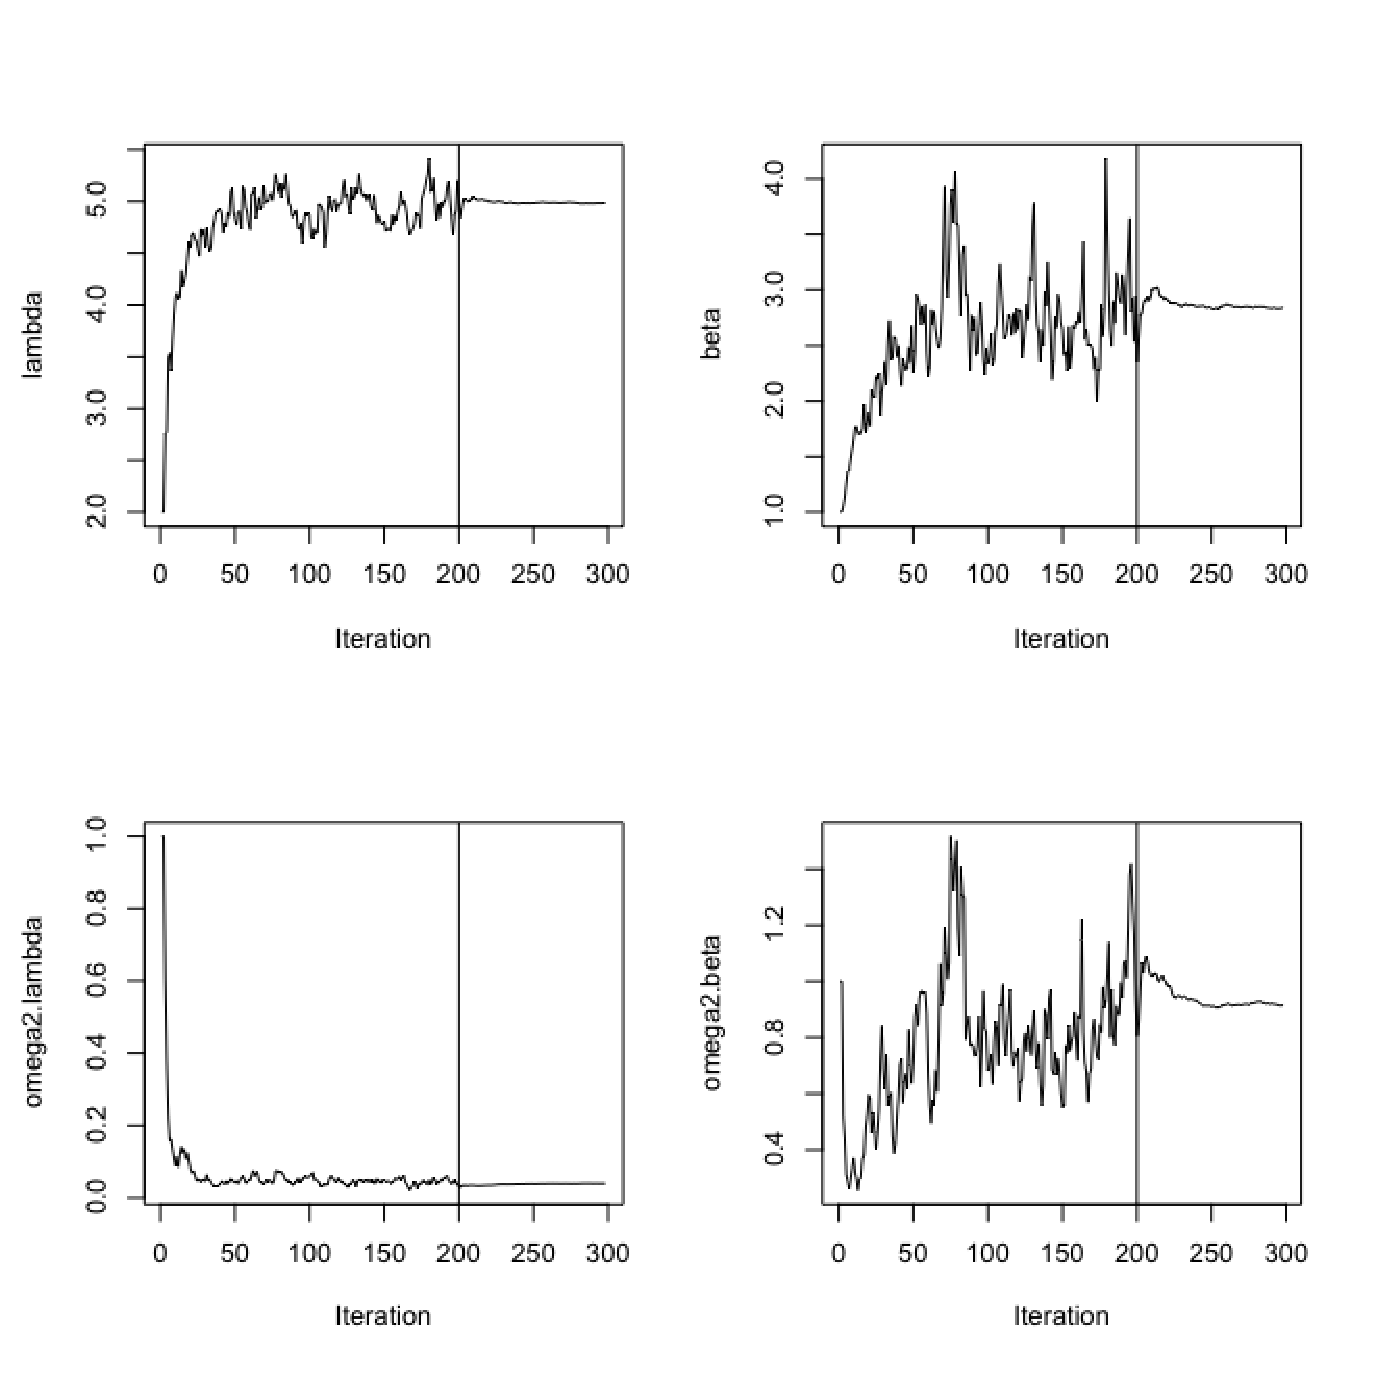
\epsfig{file=figs/popparam_tte.eps,width=9cm,angle=270}
\end{center}
\par \kern -0.5cm
\caption{Time-to-event data modelling: convergence of the empirical quantiles of order 0.1, 0.5 and 0.9 of $\dens(\psi_i | y_i ; \theta)$ for a single individual. The reference MH algorithm is in blue and the nlme-IMH is in red.} \label{fig:popTTE}
\end{figure}

